\documentclass{article}

% if you need to pass options to natbib, use, e.g.:
% \PassOptionsToPackage{numbers, compress}{natbib}
% before loading nips_2017
%
% to avoid loading the natbib package, add option nonatbib:
% \usepackage[nonatbib]{nips_2017}

\PassOptionsToPackage{numbers, compress}{natbib}
\usepackage{nips_2017}

% to compile a camera-ready version, add the [final] option, e.g.:
% \usepackage[final]{nips_2017}

\usepackage[utf8]{inputenc} % allow utf-8 input
\usepackage[T1]{fontenc}    % use 8-bit T1 fonts
\usepackage{hyperref}       % hyperlinks
\usepackage{url}            % simple URL typesetting
\usepackage{booktabs}       % professional-quality tables
\usepackage{amsfonts}       % blackboard math symbols
\usepackage{nicefrac}       % compact symbols for 1/2, etc.
\usepackage{microtype}      % microtypography

%for matrices
\usepackage{blkarray}
\usepackage{amsmath}

\usepackage{graphicx}
\usepackage{caption}
\usepackage{subcaption}

\usepackage[svgnames, table]{xcolor} % Enabling colors by their 'svgnames'

% define custom commands
\definecolor{commentPJA_color}{rgb}{1.0,0.0,0.8}
\newcommand{\commentPJA}[1]{{\textcolor{commentPJA_color}{PJA: #1}}}


% define custom commands
\definecolor{commentLP_color}{rgb}{1.0,0.0,0.8}
\newcommand{\commentLP}[1]{{\textcolor{commentLP_color}{LP: #1}}}


% define custom commands
\definecolor{commentAP_color}{rgb}{1.0,0.0,0.8}
\newcommand{\commentAP}[1]{{\textcolor{commentAP_color}{AP: #1}}}

% define custom commands
\definecolor{commentRJ_color}{rgb}{1.0,0.0,0.8}
\newcommand{\commentRJ}[1]{{\textcolor{commentRJ_color}{RJ: #1}}}


\newcommand{\mb}[1]{\mathbf{#1}}
\newcommand{\bs}[1]{\boldsymbol{#1}}
\newcommand{\mvec}[1]{\mathbf{#1}}

\title{Fully Bayesian Dimensionality Reduction Modeling with GT-PPCA}

% The \author macro works with any number of authors. There are two
% commands used to separate the names and addresses of multiple
% authors: \And and \AND.
%
% Using \And between authors leaves it to LaTeX to determine where to
% break the lines. Using \AND forces a line break at that point. So,
% if LaTeX puts 3 of 4 authors names on the first line, and the last
% on the second line, try using \AND instead of \And before the third
% author name.

\author{
  David S.~Hippocampus\thanks{Use footnote for providing further
    information about author (webpage, alternative
    address)---\emph{not} for acknowledging funding agencies.} \\
  Department of Computer Science\\
  Cranberry-Lemon University\\
  Pittsburgh, PA 15213 \\
  \texttt{hippo@cs.cranberry-lemon.edu} \\
  %% examples of more authors
  %% \And
  %% Coauthor \\
  %% Affiliation \\
  %% Address \\
  %% \texttt{email} \\
  %% \AND
  %% Coauthor \\
  %% Affiliation \\
  %% Address \\
  %% \texttt{email} \\
  %% \And
  %% Coauthor \\
  %% Affiliation \\
  %% Address \\
  %% \texttt{email} \\
  %% \And
  %% Coauthor \\
  %% Affiliation \\
  %% Address \\
  %% \texttt{email} \\
}

\begin{document}
% \nipsfinalcopy is no longer used

\maketitle

\begin{abstract}
Probabilistic PCA (PPCA) is a probabilistic generative model used for finding low dimensional representations of high-dimensional data. While PPCA is highly flexible in theory, in practice, the orthonormality constraints on the matrix parameter of PPCA makes it difficult to build complex PPCA-like models and conduct fully-Bayesian inference on them using modern algorithms like NUTS and ADVI. To address this computational challenge, we present the geometrically-motivated Givens Transform (GT) that represents orthonormal matrices in terms of unconstrained parameters. Our approach, that we refer to as GT-PPCA, allows us to rapidly build and prototype PPCA and related models in a probabilistic programming framework like Stan, opening up the possibility for fully-Bayesian inference on a wide-class of dimensionality reduction models using a variety of different inference algorithms, including NUTS and ADVI. The geometric insight provided by GT-PPCA also allows us to address previously unresolved issues arising in Bayesian dimensionality such as unidentifiability of matrix parameters and tractable hierarchical modeling of subspaces. We demonstrate these improvements and show how we use GT-PPCA in Stan (code provided) in a real-world setting to build a hierarchical subspace model of medical patients, as well as capture the low-rank time-dependent dynamics of a network of school children.
\end{abstract}

%%%%%%%%%%%%%%%%%%%%%%%%%
\section{Introduction}
%%%%%%%%%%%%%%%%%%%%%%%%%

Probabilistic PCA (PPCA) \citep{tipping1999probabilistic} posits a probabilistic generative model where high-dimensional data is determined by a linear function of some low-dimensional latent state. This generative model readily allows us to extend PPCA to describe the generative process of our data as we see fit. Notably, the PPCA generative model has been extended to obtain Sparse PCA \citep{hoff2009simulation}, Bayesian Exponential PCA \citep{mohamed2009bayesian}, Mixtures of Factor Analyzers \citep{ghahramani1996algorithm}, and Canonical Correlation Analysis (CCA) \citep[chapt.~12.5]{murphy2012machine}. This ability to extend PPCA is crucial for describing complex datasets arising in domains such as medicine where data may be stratified, consist of multiple views, or may vary over time. However, despite the demonstrated flexibility of PPCA, computational and statistical challenges that stem from the orthonormal matrix parameter of PPCA and related models stand in the way of making it a part of a routine modeling workflow. Ideally, one would be able to rapidly prototype diverse Bayesian dimensionality-reduction models in the framework of a probabilistic programming language like Stan \citep{carpenter2016stan}, and subsequently infer these models using state-of-the-art, fully-Bayesian inference algorithms like NUTS or ADVI. 

We draw on techniques from differential geometry and numerical analysis to introduce the Givens Transform, a novel representation of orthonormal matrices, that we use to easily build complex Bayesian dimensionality-reduction models in Stan. We refer to this approach applied to PPCA as GT-PPCA. We provide Stan code for GT-PPCA and other example models allowing for use and expansion by researchers and scientists out-of-the-box. We also demonstrate how we use GT-PPCA in Stan in our own applied work to model and infer real-world data arising from complex generative processes, a task that was previously difficult and inaccessible to novices due to implementation constraints, as we explain in the next section. Specifically, we show how we use Stan's NUTS algorithm to obtain fully-Bayesian posterior inferences for a hierarchical subspace model of medical patients, as well as a Hidden Markov Model (HMM) that captures the low-rank time-dependent dynamics of a network of school children.

In addition to alleviating implementation challenges of Bayesian dimensionality reduction models, the Givens Transform, which represents orthonormal matrices in terms of a sequence of fundamental rotations through given angles, yields insight into novel and useful ways to work with and interpret these models, which in turn helps address previously unresolved issues.  Specifically, the elegant geometric representation lets us see how by limiting the range of the parameters in GT-PPCA, we can naturally avoid issues of un-identifiability that arise when working with orthonormal matrices.  GT-PPCA also allows us new and creative ways to generate and use prior distributions on orthonormal matrices, and thus subspaces, a task that had previously been rather complicated due to the difficulty of evaluating densities of orthonormal matrix distributions for even small problem sizes~\citep{hoff2009simulation}.  As we shall discuss in more detail, our GT representation provides a rather natural way to specify prior distributions comparable to the Matrix Langevin prior \citep{muirhead2009aspects}.

%When first considering this problem, it may seem that this geometry may rule out a straightforward use of two of the most prominent techniques for posterior inference posterior inference, Markov Chain Monte Carlo (MCMC) and Variational Inference (VI).  Intuitively, for MCMC, we have no way of guaranteeing that a chain over $W$ will explore only valid regions of parameter space that satisfy the orthonormality constraints. Similarly for Variational Inference, positing a common variational posterior distribution such as a Gaussian over the elements of $W$ is sure to lead to posteriors that assign mass to invalid regions of parameter space.


\paragraph{Related work} While previous methods have been developed for posterior sampling of orthonormal matrices, they can at times suffer from numerical issues, are difficult to implement on large probabilistic graphical models, and are not generally adaptable to the widely available inference schemes such as NUTS or ADVI. \citet{brubaker2012family} and \citet{byrne2013geodesic} developed different approaches to modify the Leap-Frog integrator typically used in Hamiltonian Monte Carlo (HMC), so that Hamiltonian exploration, and thus MCMC samples of posteriors, satisfied any necessary constraints at all times. Specifically,~\citet{brubaker2012family} uses the SHAKE integrator \citep{leimkuhler2004simulating} to simulate Hamiltonian dynamics and generate proposals. The integrator works by repeatedly taking a step forward that may be off the manifold using ordinary leap frog, then projecting back down to the nearest point on the manifold. The projection is done via Newton iterations, which may converge to the wrong local minimum in practice or possibly not converge at all causing divergences~\citep{betancourt2017divergences}. While both of these possibilities jeopardize the ergodicity of a Markov Chain, and the integrity of samples, the former is more dangerous as it occurs without warning. On the other hand, \citet{byrne2013geodesic}~ exploit the fact that closed form solutions are known for the geodesic equations in the space of orthonormal matrices in the embedded coordinates, $W$, and use their derived Embedded Manifold HMC (EMHMC) sampler to perform posterior inference. While this method is completely explicit, requiring no Newton iterations, in practice we found that for larger step sizes, the integrator steps off the Stiefel manifold, due to the numerical imprecision of the matrix exponential function. Because these methods use modified integrators for constrained parameters, in practice they require additional book-keeping to track the support and the integrator of each variable, adding an extra layer of implementation complexity, especially for large complex models with many parameters.  This makes it difficult to implement these methods within a probabilistic programming framework such as Stan, which typically does not expose the underlying inference algorithm to the user. Unfortunately, this precludes the rapid prototyping and building of models as well as the flexibility to use different inference algorithms that Stan provides. Lastly, we remark that for inference on orthonormal matrices, these methods can lead to multi-modal posteriors, that can be avoided in a straight-forward way using the Givens transform, as we discuss in sections \ref{geomGivens} and \ref{examples}.

\paragraph{Paper outline} A brief overview of probabilistic dimensionality reduction is provided in Section~\ref{Probabilistic dimensionality reduction}. The geometry of the Stiefel Manifold is discussed in Section~\ref{geometry} and the Givens Transform (GT) is introduced in Section~\ref{Givens}. Empirical studies where GT-PPCA was used in Stan for for building complex probabilistic graphical models are presented in Section~\ref{examples}.

%%%%%%%%%%%%%%%%%%%%%%%%%

%%%%%%%%%%%%%%%%%%%%%%%%%
%%%%%%%%%%%%%%%%%%%%%%%%%
%%%%%%%%%%%%%%%%%%%%%%%%%
\section{Probabilistic Principal Component Analysis (PPCA)} \label{Probabilistic dimensionality reduction}
%%%%%%%%%%%%%%%%%%%%%%%%%
%%%%%%%%%%%%%%%%%%%%%%%%%
%%%%%%%%%%%%%%%%%%%%%%%%%

PPCA posits the following generative process for how a sequence of high-dimensional data vectors $\mathbf{x}_i \in \mathbb{R}^n$, $i = 1, \cdots, N$ arise from some low dimensional latent representations $\mathbf{z}_i \in \mathbb{R}^p$ ($p < n$):
\begin{eqnarray}
\label{eq:PpcaGenerativeProcess}
p(\mb{z}_i) &\sim& \mathcal{N}_p(0, I) \nonumber\\
p(\mb{x}_i | \mb{z}_i, W, \Lambda, \sigma^2) &\sim& \mathcal{N}_n(W \Lambda \mb{z}_i, \sigma^2 I).
\end{eqnarray}
Here $W$ is an $n \times p$ orthonormal matrix and $\Lambda$ is a $p \times p$ diagonal matrix with positive elements.  For simplicity, we have presented the case where the data has zero mean, but the more general case can also readily be considered \citep[chapt.~12.1]{murphy2012machine}. We note that in the limit of $\sigma^2$ going to zero, the maximum likelihood estimator $\hat{W}$ of $W$ converges to the matrix given by classical PCA~\citep{tipping1999probabilistic}. Inference for PPCA and extensions is usually conducted in practice by obtaining point estimates of $W$ via Expectation Maximization (EM) \citep[chapt.~12.2.5]{murphy2012machine}.

\paragraph{Extensions to PPCA}
As mentioned previously, PPCA as a generative model can be flexibly expanded in several ways to produce new models. To build a probabilistic sparse PCA, one can place a Laplace or Cauchy prior over the elements of $W$. \citet{mohamed2009bayesian} showed that we can model non-Gaussian data, $\mb{x}_i$, by replacing equation \ref{eq:PpcaGenerativeProcess} with any distribution from the exponential family whose natural parameters are given by $\mathrm{Expon}(W\Lambda \mb{z}_i)$, where $\mathrm{Expon}(\cdot)$ is an appropriate link function. \citet{ghahramani1996algorithm} use a mixture of several $W$ matrices for different regions of data space to extend PPCA to the non-linear case. GT-PPCA in the context of a probabilistic programming framework like Stan makes these extensions to the base PPCA model easy to implement, even for non-experts or people with little programming background.

\paragraph{Importance of the Orthonormality Condition}
The orthonormal constraint on the matrix $W$ plays an important role in obtaining robust methods for making inferences in probabilistic PCA because it alleviates identifiability and numerical issues.  If one were to relax the orthonormality constraint and naively conduct inference in the space of all $n\times p$ matrices, the likelihood function would assign identical probability to a whole equivalence class of matrices $W \sim V$ where the span is the same linear subspace $\mbox{span}\{W\} = \mbox{span}\{V\}$ (see \citet[chapt.~12.1.3]{murphy2012machine}).  In addition to this resulting in an unidentifiable model, in practice this presents a number of major challenges.  First, matrices in a given equivalence class are not all equally well-conditioned numerically, thus round-off errors and truncation errors become problematic in practical calculations.  Secondly, these issues with the representation further manifest in the log-likelihood objective function where regions of particularly large curvature arise, as pointed out by \citet{holbrook2016bayesian}. We note that, while most identifiability issues and numerical issues are alleviated by constraining inference to orthonormal matrices, the PPCA likelihood is equivalent for an orthonormal matrix $W$ and any permutation of the columns of $W$ being negative \citep[chapt.~12.1.3]{murphy2012machine,holbrook2016bayesian}. As such, even the methods of \citet{brubaker2012family} and \citet{byrne2013geodesic} will lead to multi-modal posteriors that can be avoided in a straightforward manner by appealing to insights revealed by the Givens Transform, as shown in Sections \ref{geomGivens} and \ref{examples}.

%\paragraph{Inference} Inference for PPCA is typically conducted by obtaining a point estimate for $W$ via a closed-form estimator, or for expanded PPCA models via (EM) \citep[chapt.~12.2]{murphy2012machine}, neither of which provide a notion of uncertainty for our point estimates. Without information regarding the uncertainty of our estimates these point estimates could be far from the true value of $W$ and thus mislead our conclusions, especially for larger models and/or when there is relatively little data available. Furthermore, point estimates do now allow for hypothesis testing e.g. statistically testing whether two different groups of observations lie in the same subspace. We show with examples how GT-PPCA in Stan makes it easy achieve these tasks in section \ref{examples}.

%%%%%%%%%%%%%%%%%%%%%%%%%
%%%%%%%%%%%%%%%%%%%%%%%%%
%%%%%%%%%%%%%%%%%%%%%%%%%
\section{Geometry of the Stiefel Manifold} \label{geometry}
%%%%%%%%%%%%%%%%%%%%%%%%%
%%%%%%%%%%%%%%%%%%%%%%%%%
%%%%%%%%%%%%%%%%%%%%%%%%%

The orthonormality of $W$ in Equation (\ref{eq:PpcaGenerativeProcess}) introduces the challenge of having to work with prior and posterior distributions over orthonormal matrices. To make better sense of these types of objects, as well as the space of orthonormal matrices we must analyze their geometric properties.

Just as three-dimensional unit vectors form a sphere in $\mathbb{R}^3$, which is a submanifold of $\mathbb{R}^3$, the set of $n\times p$ orthonormal matrices, form a sub-manifold in the space of general $n \times p$ matrices known as the Stiefel Manifold and denoted $V_{n,p}$\citep{muirhead2009aspects}. $V_{n,p}$ is formally defined as

\begin{equation}
V_{n,p} := \{Y \in \mathbb{R}^{n \times p}: YY^T = I \}.
\end{equation}

The elements of $V_{n,p}$ can be thought of as $p$-frames, a collection of $p$ orthonormal vectors that lie in $n$-dimensional space. To move about the Stiefel manfiold, one can rigidly rotate the vectors in the $p$-frame about any combination of axes an arbitrary number of times. The case where $n = 3$ and $p = 1$ corresponds to a sphere, while the case where $n = 3$ and $p = 2$, has an extra angle, $\theta_{23}$ that controls how much the second basis vector is rotated about the first (Figure \ref{fig:StiefelGeom}). Put in this perspective, for a three-dimensional set of points forming a flat, pancake-like cloud, PCA can be thought of as finding the best $2$-frame that aligns with this cloud Figure \ref{fig:MleSubspaceEstimate}.

\begin{figure}
    \centering
    \begin{subfigure}[b]{0.26\textwidth}
        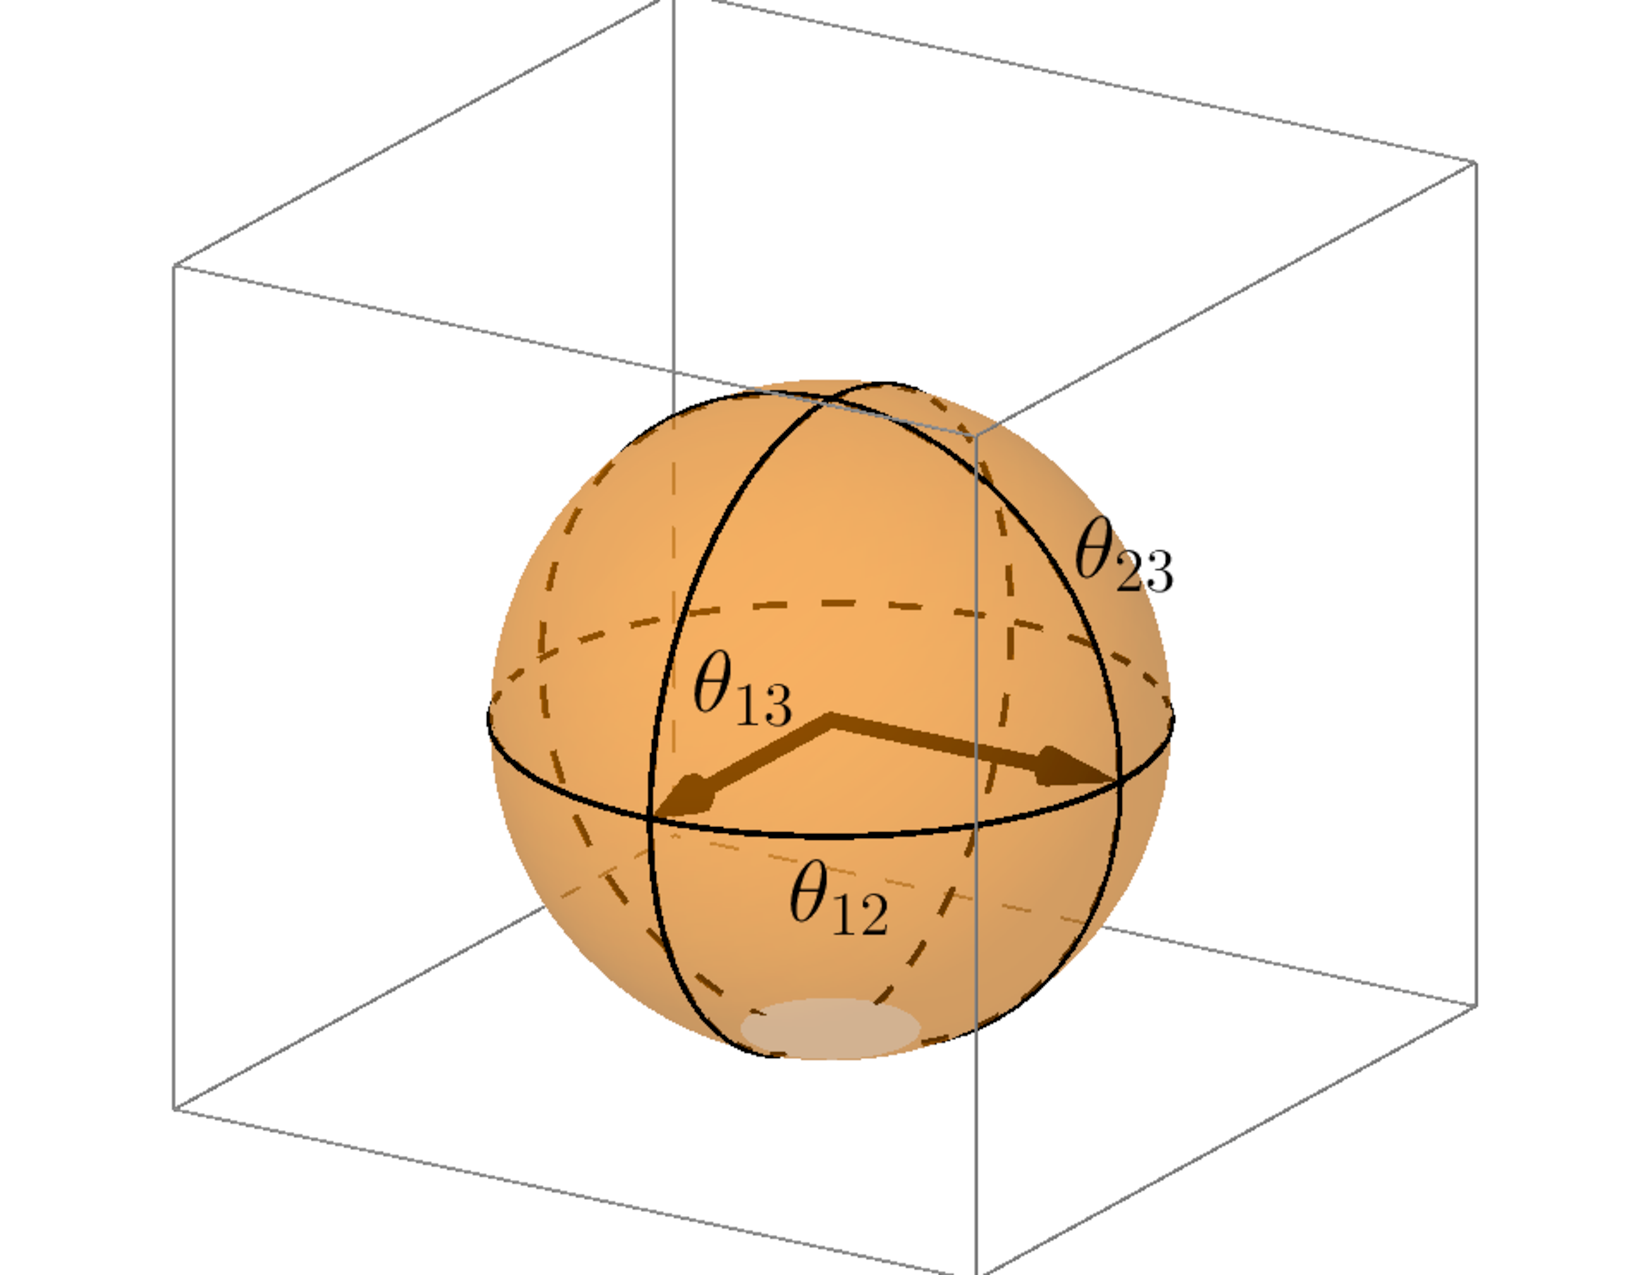
\includegraphics[width=\textwidth]{StiefelGeom.pdf}
        \caption{}
        \label{fig:StiefelGeom}
    \end{subfigure}
    ~ %add desired spacing between images, e. g. ~, \quad, \qquad, \hfill etc. 
    %(or a blank line to force the subfigure onto a new line)
    \begin{subfigure}[b]{0.25\textwidth}
        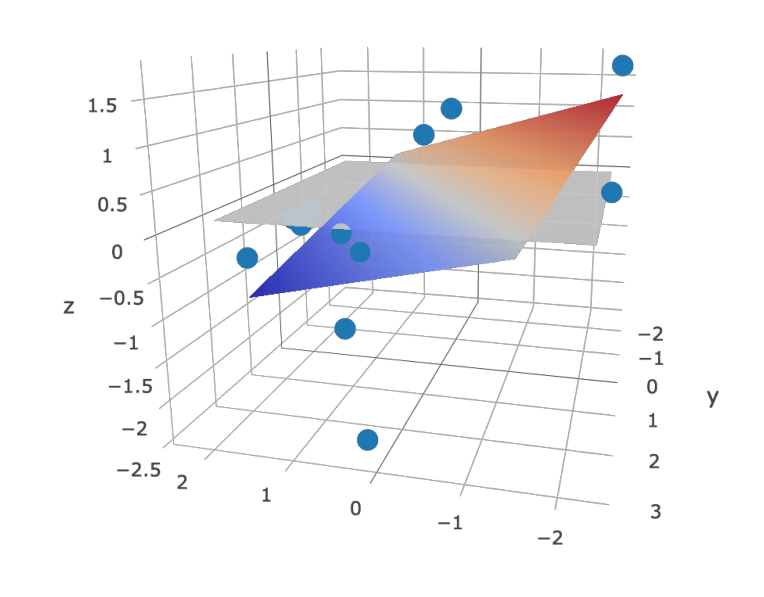
\includegraphics[width=\textwidth]{uncertainty.pdf}
        \caption{}
        \label{fig:MleSubspaceEstimate}
    \end{subfigure}
    ~ %add desired spacing between images, e. g. ~, \quad, \qquad, \hfill etc. 
    %(or a blank line to force the subfigure onto a new line)
    \begin{subfigure}[b]{0.26\textwidth}
        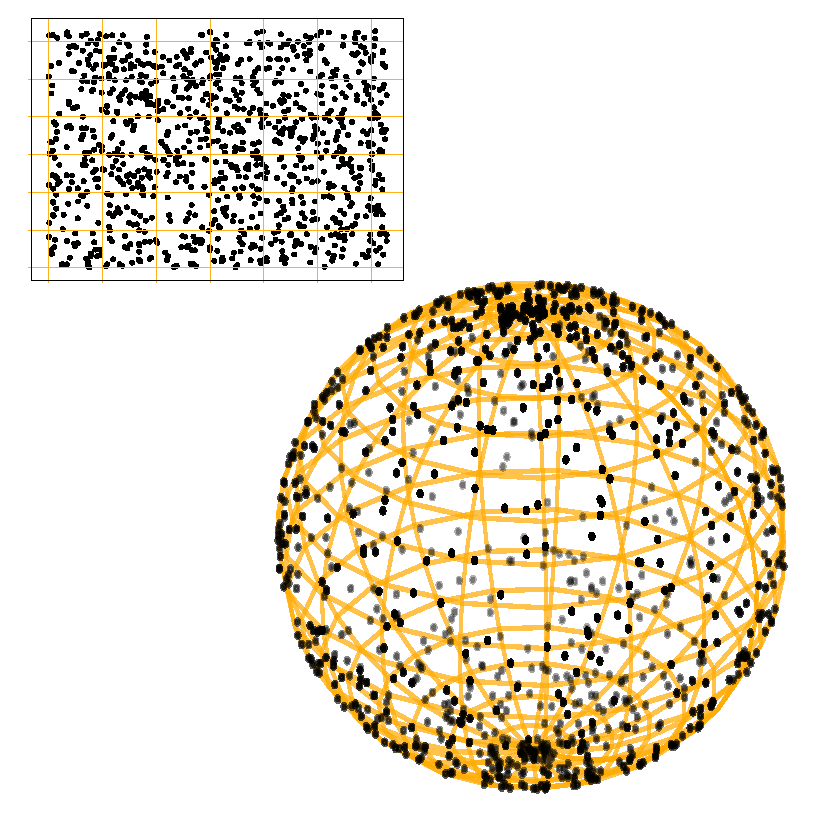
\includegraphics[width=\textwidth]{AreaForm.pdf}
        \caption{}
        \label{fig:AreaForm}
    \end{subfigure}
    \caption{Visualizing the Givens Transform. (a) To obtain different elements of the Stiefel Manifold we rigidly rotate $p$-frames. This motivates the connection to Givens Reductions which work by rotating in some plane (inset) (b) PCA finds the orthonormal matrix in the Stiefel Manifold that best describes the subspace the data lie in, although in this case the point estimates is misleads us from the true subspace, which in this case is flat. (c) Even if we sample uniformly in angle coordinates (inset), without a proper measure adjustment samples will not be uniform when transformed to the sphere. In this case, samples are sparse near the equator and congregate near the poles.}\label{fig:Givens}
\end{figure}
 
Even though $n \times p$ orthonormal matrices are typically represented by $np$ elements, the intrinsic dimension of the Stiefel Manifold, $V_{n,p}$, is actually $np-p(p+1)/2$. This arises from the constraints on the columns of the matrix that impose orthonormality.  This dimensionality can be seen by observing, that the first column of $Y \in V_{n,p}$ must have norm one and hence has one constraint placed on it. The second column must also have norm one and also must be orthogonal to the first column hence with two constraints placed on it.  Continuing to the third column through the $n^{th}$ one arrives at the conclusion that each point of the Stiefel Manifold has only $np - (1+2+\cdots+p) =np-p(p+1)/2$ degrees of freedom.  The reduced dimensionality motivates the Givens Transform, which can be thought of as an $np-p(p+1)/2$-dimensional set of coordinates $\Theta$, that represent elements of the Stiefel manifold.

%%%%%%%%%%%%%%%%%%%%%%%%%
%%%%%%%%%%%%%%%%%%%%%%%%%
%%%%%%%%%%%%%%%%%%%%%%%%%
\section{Givens Transform (GT) approach to PPCA (GT-PPCA)} \label{Givens}
%%%%%%%%%%%%%%%%%%%%%%%%%
%%%%%%%%%%%%%%%%%%%%%%%%%
%%%%%%%%%%%%%%%%%%%%%%%%%

Posterior distributions for several types of constrained parameters are routinely inferred in practice using both MCMC and VI by transforming the constrained variables to an unconstrained space. Using a smooth one-to-one mapping, $T: \mathrm{supp}(z) \to \mathbb{R}^D$, where $\mathrm{supp}(z)$ is the support of the constrained random variable $z$, one can obtain a posterior over the unconstrained parameter that corresponds to the original constrained parameter of interest, then map inferences back to the original constrained space. This procedure requires computing the Jacobian, $J_{T^{-1}}$ of the transformation, to obtain $f_{Y}(y) = f_{z}(T^{-1}(y)) J_{T^{-1}}(y)$ where $Y$ is an unconstrained random variable with probability density function (PDF) $f_Y$ and $f_{z}$ is the probability density of $z$, which for PPCA comes from (\ref{eq:PpcaGenerativeProcess}). The extra Jacobian term accounts for how the a unit volume under the transformation changes \citep{kucukelbir2014fully}. Without this extra Jacobian factor, inference between the two spaces is incomparable. As an example, in Figure \ref{fig:AreaForm}, we show that uniformly sampling in spherical coordinates (unconstrained space) does not correspond to uniformly sampling on the sphere (constrained space), unless we include an appropriate term accounting for how volumes are warped under the transformation. Intuitively, areas that are near the poles are shrunk far more than areas near the equator, so when mapped back on to the sphere, points will congregate closer to the poles of the sphere than the equator. Perfoming inference in a transformed space is most notably used in ADVI and Stan's HMC routines \citep{carpenter2016stan, kucukelbir2014fully}. To our knowledge no such transform has been proposed for orthonormal matrices.

%%%%%%%%%%%%%%%%%%%%%%%%%
\subsection{Givens Reductions and the Givens Transform}\label{GivensSub}
%%%%%%%%%%%%%%%%%%%%%%%%%
Appealing to the Givens Reduction motivates a transformation from $n \times p$ orthonormal matrices, a constrained space, to unconstrained angles, that we call the Givens Transform. The Givens Reduction is a numerical analysis technique for reducing a square matrix $A$ to upper-triangular form \citep{meyer2000matrix}. The technique works by applying a series of rotation matrices to $A$ such that elements below the diagonal are ``zeroed out" starting with the second element of the first column, and moving down the first column before zeroing out the appropriate elemnents of the subsequent columns. For example if $A$ is a $3 \times 3$ matrix and its first column is $(0.84, 0.48, 0.26)^T$, the Givens Reduction would would apply a rotation in the $(1,2)$-plane, $R_{12}^{-1}$ so as to annihilate the second element of this column producing $(0.93, 0.00, 0.26)^T$ (Figure \ref{fig:StiefelGeom} Inset). For an $n \times p$ orthonormal matrix $Y$, obtaining the Givens Reduction requires multiplication by $(n-1)+(n-2)+\cdots+(n-p) = np -p(p+1)/2$ rotation matrices each with their own respective angles. Since each rotation rigidly rotates the orthonormal columns of $Y$, they remain orthonormal, resulting in the matrix $I_{n,p}$, whose columns are the first $p$ columns of the $p \times p$ identity matrix:
\begin{equation}
\label{eq:GivensReduction}
(R_{pn}^{-1} \cdots R_{p,p+2}^{-1} R_{p,p+1}^{-1}) \cdots (R_{2n}^{-1} \cdots R_{24}^{-1} R_{23}^{-1})(R_{1n}^{-1} \cdots R_{13}^{-1}  R_{12}^{-1})Y = I_{n,p},
\end{equation}
Because rotations are invertible we can rewrite (\ref{eq:GivensReduction}) as
\begin{equation}
\label{eq:GivensRepresentation}
Y = (R_{12} \cdots R_{1n}) \cdots (R_{23} \cdots R_{2n}) (R_{p+1,n} \cdots R_{pn}) I_{n,p}.
\end{equation}
which we refer to as the Givens Representation of an orthonormal matrix $Y$. Since each of the $np -p(p+1)/2$ rotation matrices have an associated  angle $(\theta_{12} \cdots \theta_{1n}) \cdots (\theta_{23} \cdots \theta_{2n}) (\theta_{p+1,n} \cdots \theta_{pn})$, that we collectively refer to as $\Theta$, we can use these angles to represent any $n \times p$ orthonormal matrix. \textit{In this way we have reparameterized all $n \times p$ orthonormal matrices \footnote{other than a set of measure zero, that is thus negligible}, a constrained space, in terms of unconstrained angles \footnote{the angles are themselves constrained to lie in certain intervals e.g. $[0, \pi)$ but these sorts of constraints are routine to deal with using a one-to-one diffeomorphism between intervals and the real line e.g. the sigmoid transform}, using the Givens Transform $\Theta: V_{n,p} \to \mathbb{R}^{np -p(p+1)/2}$}. In a probabilistic programming framework like Stan we can treat $\Theta$ as an unknown parameter and $Y(\Theta)$ as a transformed variable, allowing us to use an orthonormal matrix in arbitrary likelihoods, such as the likelihood from (\ref{eq:PpcaGenerativeProcess}). We also mention that multiplication by rotation matrices are inexpensive to compute as they are highly sparse (especially in large dimensions) and when applied to a matrix, they only modify two rows of that matrix at a time.

%%%%%%%%%%%%%%%%%%%%%%%%%
\subsection{Geometry of the Givens Transform}\label{geomGivens}
%%%%%%%%%%%%%%%%%%%%%%%%%

We address implementation details of the Givens Transform relevant in practical use. Topologically, $V_{n,p}$ is locally equivalent to Euclidean space, but not globally equivalent, meaning it is impossible to find a one-to-one map between the Stiefel manifold and Euclidean space. Technically speaking, the Givens transform can map angles to all of $V_{n,p}$ except for a subset $S \subset V_{n,p}$ of measure zero.  In the $n=3, p=1$ case (the sphere), this corresponds to a sliver where $\theta_{12} = \pi$ and $\theta_{13} \in (-\pi/2, \pi/2)$. Since the set is of measure zero, with probability one, the orthonormal matrix that describes the true subspace our data lies in will not be in that set. 

In practice, we limit the angle $\theta_{12}$ to an interval of length $\pi$ rather than an interval of length $2\pi$ to avoid superfluous modes in our posterior. This is useful both for interpretation and in higher dimensional problems where the number of modes grows exponentially. Examining the angles of the Givens transform reveals how geometrically, two matrices whose columns may be the negation of each other can both be reached. Because these matrices will have equivalent likelihoods under Equation \ref{eq:PpcaGenerativeProcess}, infering over the full range of angles results in a multi-modal posterior that makes sampling and VI more difficult to perform and interpret. To avoid this multi-modality using the modified integrator methods would require a mechanism to avoid boundaries, which are not as intuitively defined in the default embedded coordinates as in the Givens transform.

Lastly, we note that if the true basis lies near a pole, i.e. $\theta_{ij}$ is close to $-\pi/2$ or $\pi/2$, then posteriors will tend to be multi-modal as the region in parameter space close to the boundaries will be nearly equally valid, while the region near zero, will not be valid and thus contain little probability mass. In these cases, one can simply change the coordinate bounds (chart) so that $\theta_{ij} \in (0, \pi)$ will have a uni-modal posterior in the new coordinate system, alleviating numerical issues. In Stan this is straightforward, as one simply has to change the lower and upper bound of the angle parameter.

\paragraph{An analogous Jacobian term using differential forms} As stated earlier, performing inference on a transform space requires a Jacobian term accounting for how volumes are warped by the transform, but in the case of the Givens Transform this poses a problem because an $n \times p$ orthonormal matrix is $np$-dimensional and the Givens transform, $\Theta(Y)$, maps this set to an $np - p(p+1)2$-dimensional set of angles $\Theta$. In this more general scenario, one can not simply take the determinant of the Jacobian as the volume morphing factor, because the Jacobian is not square and hence the determinant is undefined. To obtain the correct factor one must appeal to the calculus of differential forms. For accessibility, we provide psuedo-code in the supplementary materials, as well as actual Stan code to illustrate how one actually computes a differential form on a computer.

Differential forms measure how a transform warps an infinitesimal volume from one space to another, and they can be applied irrespective of the coordinates we use to describe either space. For example, spherical coordinates $(\theta, \varphi) \mapsto (x(\theta,\varphi), y(\theta,\varphi), z(\theta,\varphi))$ map points in the flat plane, $\mathbb{R}^2$, to points in $\mathbb{R}^3$ that lie on the sphere. $d\theta \wedge d\varphi$ represents a small area in the plane that can be rewritten as a small patch in $\mathbb{R}^3$ by finding $d\theta$ and $d\varphi$ in terms of $dx, dy$, and $dz$ and applying the well defined rules of a wedge product. For a thorough account we recommend \citet{muirhead2009aspects}, \citet{edelman200518}, or any standard text in differential geometry.

We can analogously use differential forms and wedge products to measure volumes on the Stiefel manifold. For $n \times p$ orthonormal matrices, there are only $np-p(p+1)/2$ free parameters and so the proper form to measure sets of orthonormal matrices is a $np-p(p+1)/2$-form. For an orthonormal, $n \times p$ matrix, $Y$, we can find an orthonormal $n \times n$ matrix $G$ such that $G^T Y = I_{n,p}$. In fact $G$ just comes from the product of the appropriate rotation matrices that arises in the Givens Reduction (Equation \ref{eq:GivensReduction}). \citet{muirhead2009aspects} shows that the correct form for measuring volumes on the Stiefel manifold comes from wedging the elements of the $n \times p$ matrix $G^T dY$ that lie below the diagonal i.e.
\begin{equation}
\label{eq:WedgeForm}
\bigwedge_{i=1}^p \bigwedge_{j=i+1}^n G_j^T\, dY_i
\end{equation}
where $G_j$ is the $j$th column of $G$ and $Y_i$ is the $i$th column of $Y$. To obtain the form in angle coordinates, we obtain $dY_i$ in terms of the angle coordinates by the following relationship, $dY_i = J_{Y_i}(\Theta)\, d\Theta$, where $J_{Y_i}$ is the Jacobian of $Y_i$ with respect to the angle coordinates. Once we obtain the form (\ref{eq:WedgeForm}) in terms of the angle coordinates, the result is a wedge product of $np-p(p+1)/2$ vectors that are $np-p(p+1)/2$ dimensional, which reduces to the determinant of these vectors aligned side by side as a $np-p(p+1)/2 \times np-p(p+1)/2$ matrix. This determinant is analogous to and serves the same purpose as Jacobian adjustment that comes from transforming random variables. We can insert it in to the log-probability of a model to avoid the sort of unintended sampling behavior depicted in Figure \ref{fig:AreaForm}. We incorporate the form (\ref{eq:WedgeForm}) in to the log-probability of all of our Stan examples.

%%%%%%%%%%%%%%%%%%%%%%%%%
%%%%%%%%%%%%%%%%%%%%%%%%%
%%%%%%%%%%%%%%%%%%%%%%%%%
\section{Empirical Studies} \label{examples}
%%%%%%%%%%%%%%%%%%%%%%%%%
%%%%%%%%%%%%%%%%%%%%%%%%%
%%%%%%%%%%%%%%%%%%%%%%%%%

%%%%%%%%%%%%%%%%%%%%%%%%%
\subsection{Synthetic Data}
We apply GT-PPCA in Stan to a synthetic dataset to show how GT-PPCA naturally avoids multi-modal posteriors and provides plug-and-play access to Stan's powerful NUTS implementation. We generated a synthetic, three-dimensional dataset that lies on a two-dimensional plane with $N =15$ observations according to \ref{eq:PpcaGenerativeProcess} (data is pictured in Figure \ref{fig:MleSubspaceEstimate}). We chose $\mathrm{diag}(\Lambda) =\mathrm{diag}(1, 1)$, $\sigma^2 = 1$, and $W$ to be $I_{3,2}$, which in the Givens representation corresponds to $\theta_{12} = \theta_{13} = \theta_{23} = 0$ i.e. the flat plane (Figure \ref{fig:MleSubspaceEstimate}). Our Stan code simultaneously provides posterior samples in both the $W$ coordinates and the Givens angle coordinates. Examining posterior samples of the angle coordinates elucidates GT-PPCA's avoidance of superfluous modes, as compared to EMHMC (Figure \ref{fig:multiModal}).
\begin{figure}
    \centering
    \begin{subfigure}[b]{0.38\textwidth}
        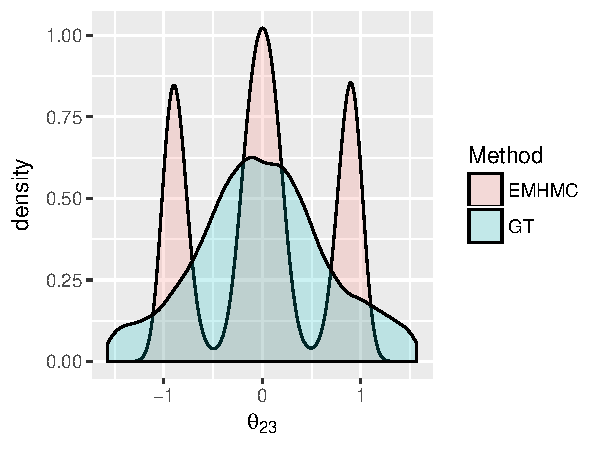
\includegraphics[width=\textwidth]{multiModal.pdf}
        \caption{}
        \label{fig:multiModal}
    \end{subfigure}
    ~ %add desired spacing between images, e. g. ~, \quad, \qquad, \hfill etc. 
      %(or a blank line to force the subfigure onto a new line)
    \begin{subfigure}[b]{0.38\textwidth}
        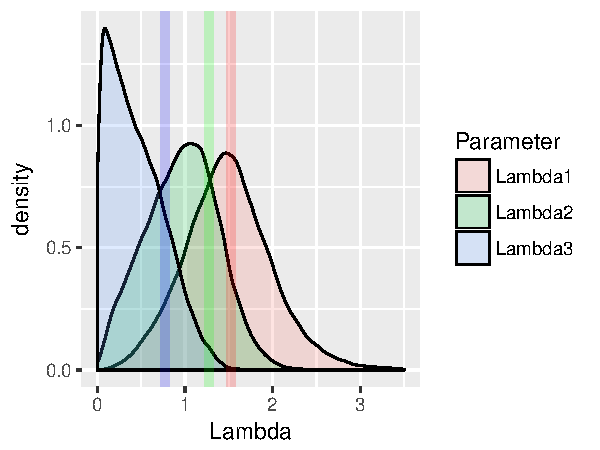
\includegraphics[width=\textwidth]{syntheticLambdaPosterior.pdf}
        \caption{}
        \label{fig:SyntheticPosteriorEstimates}
    \end{subfigure}
    \caption{Inferences for three-dimensional synthetic data. (a) By limiting the angle of rotation in GT-PPCA we can avoid the un-identifiability in our problem and eliminate multi-modal posteriors that show up in related methods. (b) Posterior draws from NUTS show that the third singular value, $\Lambda_3$ has a posterior that concentrates close to zero, indicating our model is most likely not three-dimensional given the data we have seen.}
\end{figure}
Posterior samples of $\theta_{13}$, which if we recall from Figure \ref{fig:StiefelGeom} is the Givens Transform angle that controls the upwards tilt of the plane, yields a median value of -0.24 and a 95\% posterior interval of $(-1, 0.78)$, a wide range that is indicative of a lack of certainty given our data. Meanwhile, classical PCA yields the point estimate $\hat{\theta}_{13} = -0.15$, an estimate which in this case is overfit to the data (Figure \ref{fig:multiModal}). 

The fully Bayesian approach provided by GT-PPCA in Stan also allows us to examine posterior draws of $\Lambda$ in Equation \ref{eq:PpcaGenerativeProcess} to make probabilistic statements about the inherent dimensionality in our data. The posterior of $\Lambda_3$ for example places considerable mass close to zero (58\% of samples were less that 0.5), providing strong evidence that our data is inherently two, not three, dimensional (Figure \ref{fig:SyntheticPosteriorEstimates}). In comparison, the standard classical PCA analysis yields the singular values $\mathrm{diag}(\hat{\Lambda}) = (1.52,\, 1.27,\, 0.77)$, possibly, but ambiguously, suggesting that our data lie close to some two-dimensional plane, if one uses the heuristic that the third singular value has a larger drop off from the first two than the second has from the first.

%%%%%%%%%%%%%%%%%%%%%%%%%
\subsection{Hierarchical subspace models for grouped multi-view medical data}
%%%%%%%%%%%%%%%%%%%%%%%%%
We modeled grouped multi-view hospital data for injured patients using a hierarchical CCA model~\citep[chapt.~15.2]{murphy2012machine}. CCA can model two types (or views) of data as being a function of two respective latent low dimensional states, but also a common latent state that captures the common information contained in both view. In our case we compared blood protein measurements and clot strength measurements for injured patients belonging to one of four groups depending on the type of injury they had. While the four types of injuries were different enough so that we could not use a single CCA model to capture the characteristics of all models at once, the four groups were not so different as to warrant separate CCA models for each. To share information between the CCA models we placed a hierarchical prior over the orthonormal matrices belonging to the distinct CCA parameters of each group (Figure \ref{fig:CCA}).

\begin{figure}
    \centering
    \begin{subfigure}[b]{0.35\textwidth}
        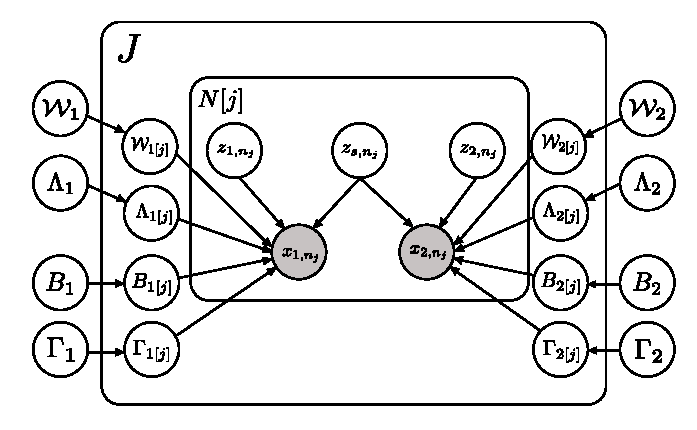
\includegraphics[width=\textwidth]{CCA.pdf}
        \caption{}
        \label{fig:CCA}
    \end{subfigure}
    ~ %add desired spacing between images, e. g. ~, \quad, \qquad, \hfill etc. 
      %(or a blank line to force the subfigure onto a new line)
    \begin{subfigure}[b]{0.35\textwidth}
        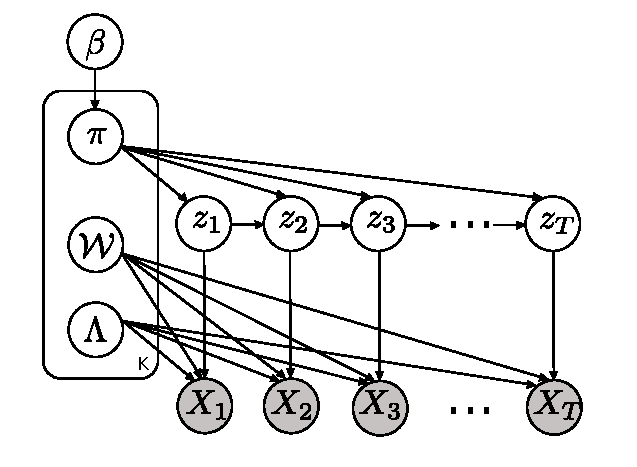
\includegraphics[width=\textwidth]{HMM.pdf}
        \caption{}
        \label{fig:HMM}
    \end{subfigure}
    \caption{Probabilistic graphical models for (a) Hierarchical CCA Model (b) Network HMM.}\label{fig:ccaResults}
\end{figure}

While distributions on the Stiefel Manifold such as the Matrix Langevin distribution \citep{muirhead2009aspects} exist, these distributions are difficult to use in practice, as computing their density requires evaluating an expensive matrix sum \citep{hoff2009simulation}. By appealing to the Givens Transform and placing a hierarchical prior over the angles of the different orthonormal matrices, we were able to build a hierarchical model over subspaces, a previously intractable task. The hierachical prior ``shrinks" the posterior median of the orthonormal matrices towards a common mean in addition to reducing the variance of these estimates (Figure \ref{fig:nonHierPosteriors,fig:hierPosteriors}). This is particularly helpful for groups with only a smaller number of observations such as the SW group, which only contains 16 patients in comparison of the GSW group with 86 patients. Comparing the angle between the first principal components for the SW and GSW group illustrates how using a hierarchical prior shrinks estimates of subspaces together towards a common hierarchical subspace (Figure \ref{fig:ccaResults}).

\begin{figure}
    \centering
    \begin{subfigure}[b]{0.22\textwidth}
        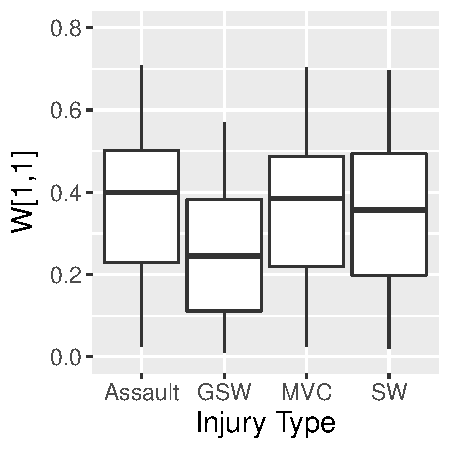
\includegraphics[width=\textwidth]{shrinkageSep.pdf}
        \caption{}
        \label{fig:nonHierPosteriors}
    \end{subfigure}
    ~ %add desired spacing between images, e. g. ~, \quad, \qquad, \hfill etc. 
      %(or a blank line to force the subfigure onto a new line)
    \begin{subfigure}[b]{0.22\textwidth}
        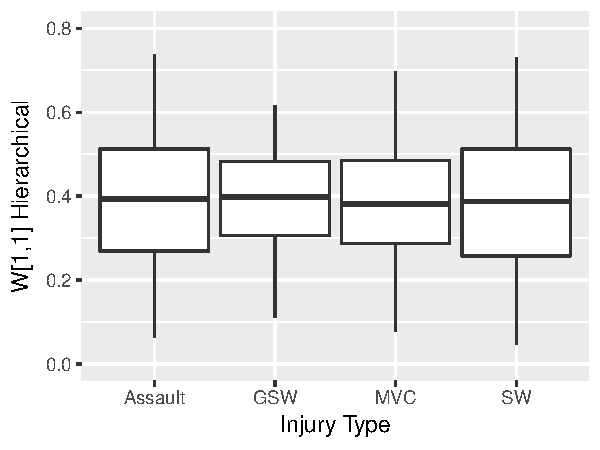
\includegraphics[width=\textwidth]{shrinkageHier.pdf}
        \caption{}
        \label{fig:hierPosteriors}
    \end{subfigure}
    ~ %add desired spacing between images, e. g. ~, \quad, \qquad, \hfill etc. 
    %(or a blank line to force the subfigure onto a new line)
    \begin{subfigure}[b]{0.37\textwidth}
        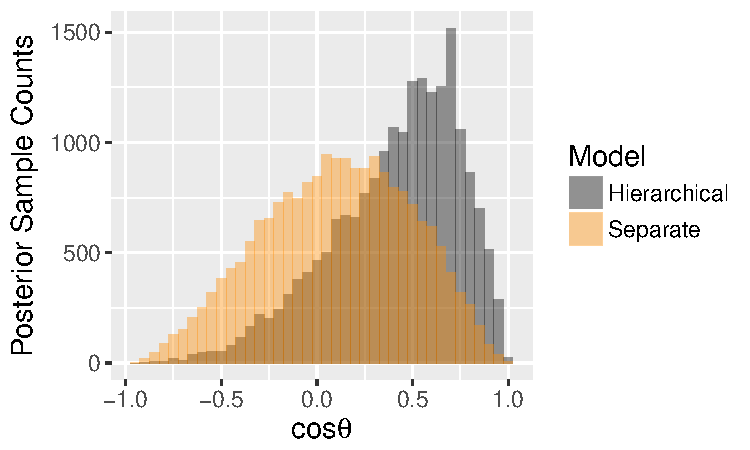
\includegraphics[width=\textwidth]{posteriorCosAngle.pdf}
        \caption{}
        \label{fig:posteriorCosAngle}
    \end{subfigure}
    \caption{Inferences for Hierarchical CCA model. (a) When estimated separately estimates of the matrix parameter $W$ have high uncertainty. (b) Placing a hierarchical prior over these matrices with GT-PPCA shrinks these parameter to a common hierarchical mean and results in smaller posterior intervals. (c) Geometrically the respective first principal component of two different groups are shrunk closer together in a hierarchical model.}\label{fig:ccaResults}
\end{figure}

%%%%%%%%%%%%%%%%%%%%%%%%%
\subsection{School Network}
%%%%%%%%%%%%%%%%%%%%%%%%%
We built an HMM subspace for count data to model the hidden time-dependent structure of a network of school children. RF sensors were used to track the interactions between school children in 12 different classes (two classes for grades 1-6) for an entire school day so as to better understand how disease spreads throughout a network \citep{stehle2011high}. We collated the number of interactions between each pair of classes in to 11-minute contiguous time windows, giving us 177 symmetric matrices of counts representing the network structure between the different classes throughout the whole day (Figure \ref{fig:heatmap}, lower row). We modeled the elements of these count matrices as each coming from a Poisson distribution whose rate comes from the element-wise exponential of a symmetric matrix $R = \exp (W \Lambda W^T)$, where the orthonormal matrix $W$ captures the low-dimensional structure of the network. To model the time varying structure of the network, we posited that the network was always in one of three latent states, that evolve according to a Markov Chain (Figure \ref{fig:HMM}). The three states each have their own associated orthonormal matrix $W_i$ that captures the low-dimensional latent network structure for that state.

\begin{figure}
    \centering
    \begin{subfigure}[b]{0.28\textwidth}
        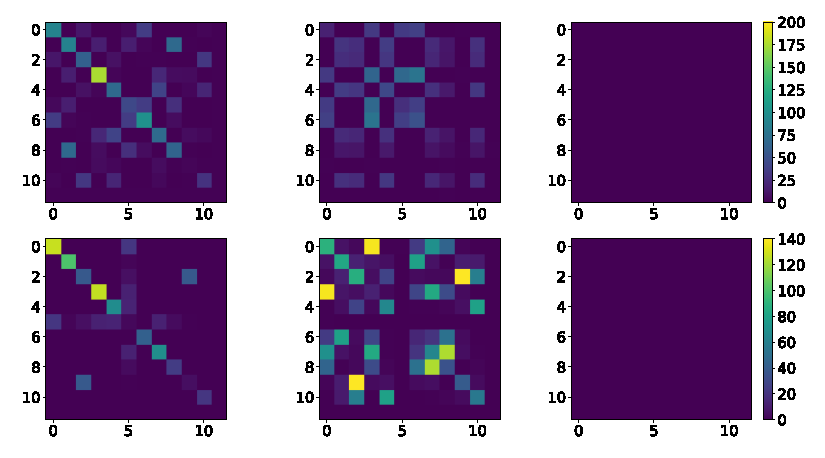
\includegraphics[width=\textwidth]{heatmap.pdf}
        \caption{}
        \label{fig:heatmap}
    \end{subfigure}
    ~ %add desired spacing between images, e. g. ~, \quad, \qquad, \hfill etc. 
      %(or a blank line to force the subfigure onto a new line)
    \begin{subfigure}[b]{0.21\textwidth}
        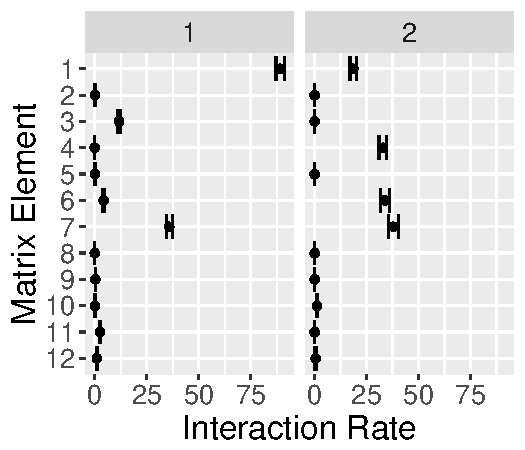
\includegraphics[width=\textwidth]{SchoolRateMatrix.pdf}
        \caption{}
        \label{fig:SchoolRateMatrix}
    \end{subfigure}
    ~ %add desired spacing between images, e. g. ~, \quad, \qquad, \hfill etc. 
      %(or a blank line to force the subfigure onto a new line)
    \begin{subfigure}[b]{0.21\textwidth}
        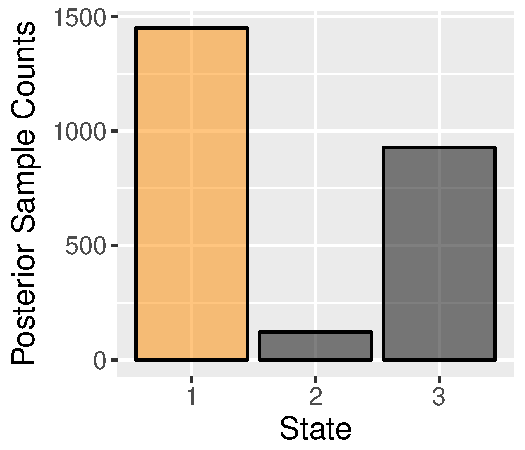
\includegraphics[width=\textwidth]{SchoolStatePosterior.pdf}
        \caption{}
        \label{fig:SchoolStatePosterior}
    \end{subfigure}
    \caption{(a) Posterior modes of rate matrices for the three states (top) capture the pattern found in example count matrices belonging to each of these three states (bottom). (b) Posterior intervals from GT-PPCA with NUTS capture uncertainty in the orthonormal matrix estimates for the first two columns of the rate matrix for the first hidden state. (c) Posterior draws can tell us the posterior probability that the network was in a certain state given the data.}
\end{figure}

Posterior modes capture the latent structure of the rate matrices of the three hidden state (Figure \ref{fig:heatmap} top row), while NUTS sampling in Stan provides full Bayesian posteriors for each of the elements of these rate matrices (Figure \ref{fig:SchoolRateMatrix}). Stan also allows us to generate samples from posterior samples of the Markov Chain, allowing us to provide a posterior over which of the hidden states the network is in at a given time (Figure \ref{fig:SchoolStatePosterior}), a common inference task in disease networks as well as fMRI networks.


%%%%%%%%%%%%%%%%%%%%%%%%%
%%%%%%%%%%%%%%%%%%%%%%%%%
%%%%%%%%%%%%%%%%%%%%%%%%%
\section{Discussion}
%%%%%%%%%%%%%%%%%%%%%%%%%
%%%%%%%%%%%%%%%%%%%%%%%%%
%%%%%%%%%%%%%%%%%%%%%%%%%
We introduced the Givens Transform as a theoretical representation of orthonormal matrices as well as a practical tool for building complex Bayesian dimensionality-reduction models in a probabilistic framework like Stan. We showed using real-world examples how GT-PPCA allows out-of-the-box usage of Stan's powerful suite of inference algorithms, as well as other practical benefits such as avoidance of multi-modal posteriors and access to new types of useful distributions using the angle representation. We provide Stan code for GT-PPCA and our other models allowing for fully Bayesian dimensionality reduction analysis without any implementation hassle.

\subsubsection*{Acknowledgments}

Use unnumbered third level headings for the acknowledgments. All
acknowledgments go at the end of the paper. Do not include
acknowledgments in the anonymized submission, only in the final paper.

%%%%%%%%%%%%%%%%%%%%%%%%%
%%%%%%%%%%%%%%%%%%%%%%%%%
%%%%%%%%%%%%%%%%%%%%%%%%%
\bibliographystyle{plainnat} % or try abbrvnat or unsrtnat
\bibliography{paperDatabase} % refers to example.bib


\end{document}
